\subsection{Specifying the boundary conditions correctly}

It can be confusing to get all the boundary conditions correct. To help you 
do this you should plot the grid and display the boundaries coloured by
the boundary condition number (this is the default) as shown in
figure~(\ref{fig:pipesBC}). In 3D you will need to
{\tt 'plot shaded surfaces'} to see the boundary colours.
This will help you see if all the faces are correct. Cgins prints out the 
number that corresponds to each boundary.
\begin{figure}[hb]
\begin{center}
  % \epsfig{file=\obFigures/pipes.bc.ps,width=.8\linewidth}  \\
  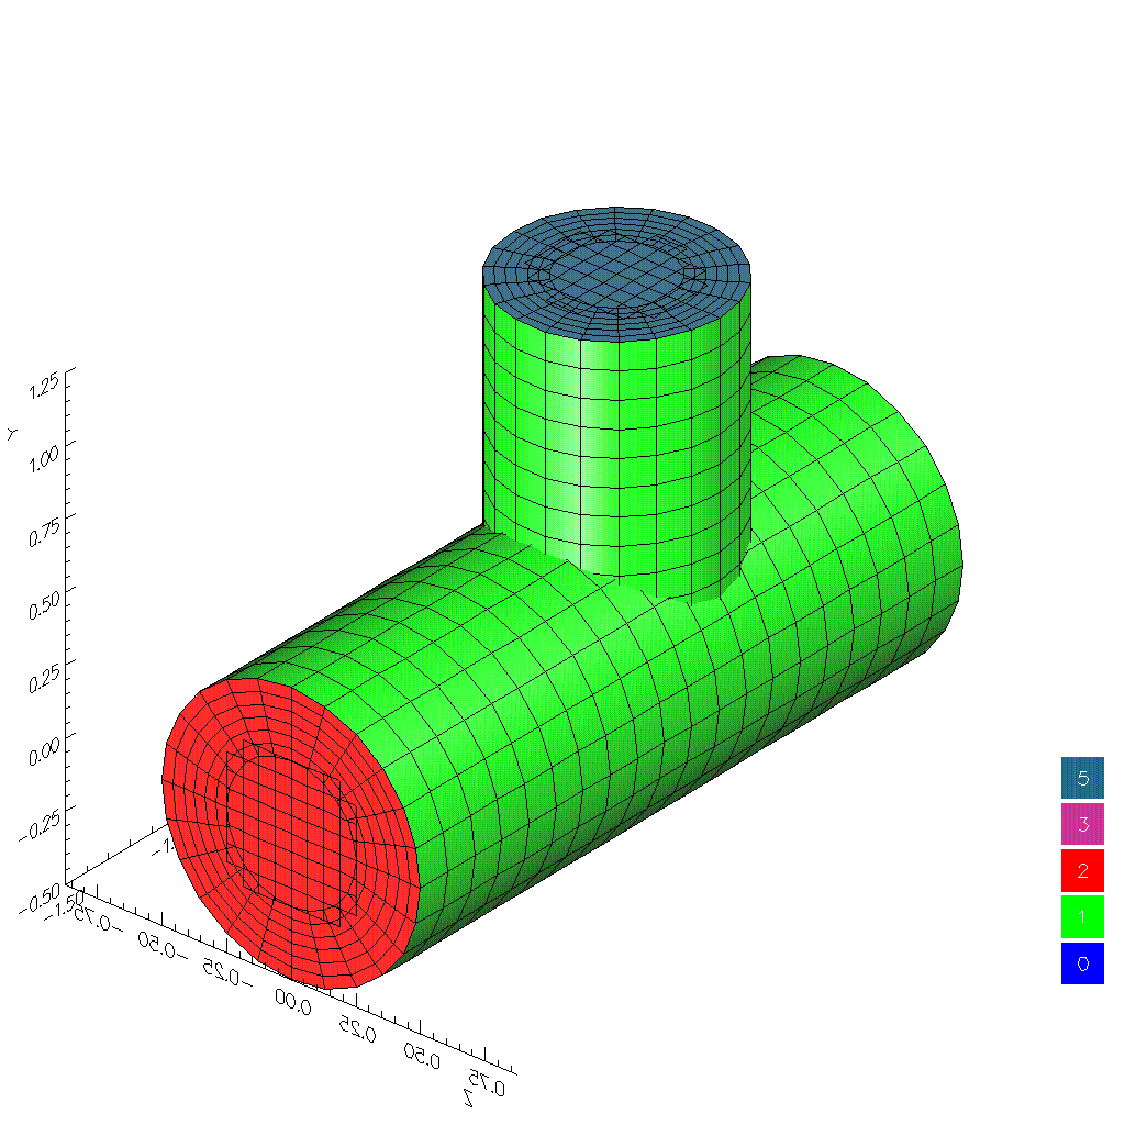
\includegraphics[width=.8\linewidth]{\insDocDir/fig/pipes_bc}
 \caption{After specifying boundary conditions it is helpful to plot the grid with
    boundaries coloured by the boundary condition number. Here we see that the
    inflow boundary for the main pipe is number 2 ({\tt inflowWithVelocityGiven})
    the outflow boundary for the branch pipe is number 5 ({\tt outflow}) and the
   walls are number 1 ({\tt noSlipWall}). This figure is best seen in {\bf colour}.}
   \label{fig:pipesBC}
\end{center}
\end{figure}
